\documentclass[12pt]{article}
\usepackage{amsmath}
\usepackage{array}
% \usepackage{gensymb}
\usepackage{geometry}
\usepackage{graphicx}
\usepackage{pgfplots}
\usepackage{siunitx}
\usepackage{wrapfig}

\title{Homework \#10}
\author{Donald Aingworth IV}
\date{October 30, 2024}

\pgfplotsset{width=8cm,compat=1.9}
\usepgfplotslibrary{external}
% \tikzexternalize

\begin{document}

\DeclareSIUnit{\mile}{mi}
\DeclareSIUnit{\gal}{gal}
\DeclareSIUnit{\foot}{ft}
\DeclareSIUnit{\h}{h}

\maketitle

\pagebreak
\section*{Problem 1}
A 1.95-kg particle is projected with an initial speed of 4.00 m/s along a surface for which $\mu_k = 0.600$.
Find the distance it travels given that: (a) the surface is horizontal; (b) the particle moves up a 30\unit{\degree} incline;
(c) the particle moves down a 30\unit{\degree} incline.

\subsection*{Solution}

\pagebreak
\section*{Problem 2}
\begin{wrapfigure}{r}{0.35\textwidth}
    \vspace{-30pt}
    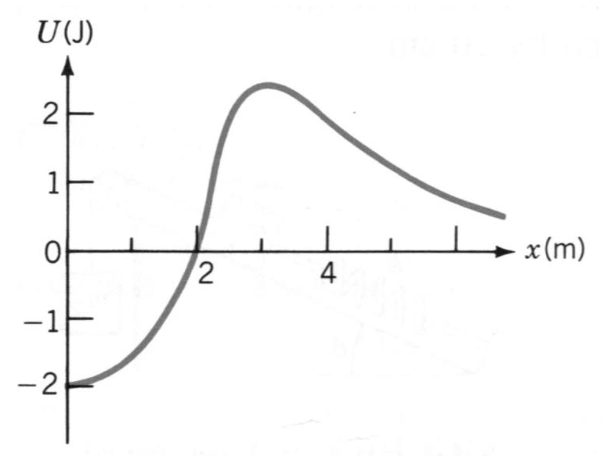
\includegraphics[width=0.35\textwidth]{graph_2.png} 
    % \label{fig:wrapfig}
\end{wrapfigure}

\subsection*{Solution}


\end{document}